\documentclass[11pt]{article}
\usepackage{amsmath, amssymb}
\usepackage{geometry} % see geometry.pdf on how to lay out the page. There's lots.
\geometry{a4paper} % or letter or a5paper or ... etc
\usepackage{graphicx}
% \geometry{landscape} % rotated page geometry
% See the ``Article customise'' template for come common customisations
\usepackage[style=phys,
citestyle=phys]{biblatex}
\addbibresource{van_vleck_memo_A.bib}

\usepackage{listings}

\title{Implementation of Van Vleck Correction for the MWA}
\author{Pyxie Star}
% delete this line to display the current date
\renewcommand{\Re}{\operatorname{Re}}
\renewcommand{\Im}{\operatorname{Im}}
%%% BEGIN DOCUMENT
\begin{document}

\maketitle
% \section{Introduction}
\paragraph{}Quantization in the MWA digital signal pathway introduces non-linear artifacts into the data. Formulae for correcting these artifacts with a Van Vleck correction were presented in \cite{VV}. An implementation of the correction has been written into \texttt{pyuvdata} as an option when reading raw MWA correlator output files. This memo describes MWA quantization, re-derives the correction formulae, and discusses the implementation.
\section{MWA Quantization}
\paragraph{}
Quantization occurs in 3 stages of the MWA digital signal pathway, twice in the digital receivers and then in the correlator. It is this final quantization that the implemented Van Vleck correction addresses. All three quantization stages are described below in a summary of the digital signal pathway.
\paragraph{}
The analog signal from a tile is attenuated to $\pm1$ Volt, and a bandpass is applied to limit the frequency range to 80-300 MHz. This signal then goes to a digital receiver, described in \cite{rec}, where it is sampled at 655.36 MHz and quantized to 8-bit values. The quantized data is then cast from real to complex, and also channelized into 256 1.28 MHz 'coarse' channels, by a polyphase filter bank (PFB). The PFB has an 8 tap subfilter followed by a 512 point FFT, and functions as follows. A Kaiser windowing function is applied to 4096 data samples. The 4096 windowed samples are split into 8 'phases' of 512 samples each, which are summed to result in 512 inputs to the FFT. The FFT outputs 256 complex values each consisting of a 16-bit real and 16-bit imaginary pair. Since each frequency channel is complex, that is, carrying two sampled values, the sampling rate is halved to 327.68 MHz. The incoming data is then shifted by 512 samples and the PFB procedure applied to this next grouping. After the FFT, a gain is applied to the data, and the second quantization occurs, taking the 16-bit real, 16-bit imaginary pair to a 5-bit real, 5-bit imaginary pair. For each observing session, some subset of 24 coarse channels are chosen and sent to the correlator. 
\paragraph{}
The MWA correlator has two stages: a PFB which channelizes the data, and a cross-multiply and accumulate module to perform the correlations. The correlator PFB  has 12-tap subfilter followed by a 128-point FFT, applying a Hanning window to the data stream. Outputs of this second PFB are quantized to 4-bit real, 4-bit imaginary pairs, and these integers are cast to floats for input into the cross-multiply. The correlator is described in greater detail in \cite{corr}, and its PFB described in \cite{pfb}.
\section{Van Vleck Correction}
\begin{figure}
\centering{}
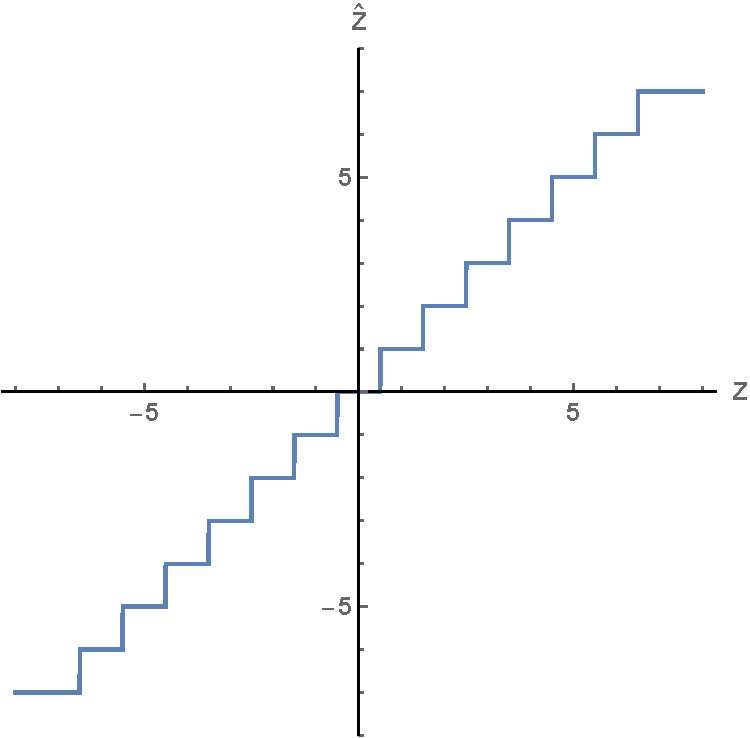
\includegraphics[width=80mm]{quant.pdf}
\caption{The 4-bit quantization pattern of the MWA.\label{quant}}
\end{figure}
\paragraph{}
The final 4-bit quantization in the correlator is assumed to have a dominant impact, and so is addressed by the Van Vleck correction.
That is, we effectively treat the values in the 4-bit quantization as being drawn from an analog zero-mean Gaussian distribution, ignoring the intermediate signal processing stages. Let $Z$ be the analog signal from an antenna and $\hat Z$ the quantized signal. The quantization pattern $\hat Z(Z)$ is shown in figure~\ref{quant}; essentially, all $Z$ values within a certain range are placed into a certain quantization bin. After correlation, we no longer have access to $\hat Z$, and so the Van Vleck correction instead treats the statistics of $\hat Z$, assuming that we are in a regime in which we can approximate the auto and cross correlations as measuring variances and covariances as described in section 3. 
\paragraph{}
First, consider the relation between the variance of $\hat Z$ and the variance of $Z$. Following \cite{VV}, the variance $E[\hat Z^2]$ is related to the probability of $Z$ falling into each of the quantization bins as follows
\begin{equation}
\begin{split}
E[\hat Z^2]=&0^2\cdot P(-0.5<Z<0.5) +(-1)^2\cdot P(-1.5<Z<-0.5)+1^2\cdot P(0.5<Z<1.5)+\cdot\cdot\cdot\\
&+(-7)^2\cdot P(Z<-6.5)+7^2\cdot P(Z>6.5)\\
=&0^2\cdot P(-0.5<Z<0.5)+1^2\cdot[P(-1.5<Z<1.5)-P(-0.5<Z<0.5)]+\cdot\cdot\cdot\\
&+7^2\cdot[1-P(-6.5<Z<6.5)]
\end{split}
\end{equation}
where we have taken advantage of the symmetry of the distribution of $Z$. With $Z$ drawn from a Gaussian distribution, the probability that $Z\in[-a,a]$
\begin{equation}
P(Z\in[-a,a])=\textrm{erf}\left(\frac{a}{\sigma_Z\sqrt{2}}\right)
\end{equation}
where $\sigma_Z$ is the standard deviation of $Z$. Combining terms gives
\begin{align}
E[\hat Z^2]=&0^2\cdot\textrm{erf}\left(\frac{0.5}{\sigma_Z\sqrt{2}}\right)+1^2\cdot\left[\textrm{erf}\left(\frac{1.5}{\sigma_Z\sqrt{2}}\right)-\textrm{erf}\left(\frac{0.5}{\sigma_Z\sqrt{2}}\right)\right]+\cdot\cdot\cdot+7^2\cdot\left[1-\textrm{erf}\left(\frac{6.5}{\sigma_Z\sqrt{2}}\right)\right]\nonumber\\
=&(-1)\textrm{erf}\left(\frac{0.5}{\sigma_Z\sqrt{2}}\right)+(-3)\textrm{erf}\left(\frac{1.5}{\sigma_Z\sqrt{2}}\right)+\cdot\cdot\cdot+(-13)\textrm{erf}\left(\frac{6.5}{\sigma_Z\sqrt{2}}\right)+7^2\nonumber\\
=&7^2-\sum_{k=0}^6(2k+1)\textrm{erf}\left(\frac{k+0.5}{\sigma_Z\sqrt{2}}\right).
\end{align}
This result can be written in terms of the standard deviation of $\hat Z$:
\begin{equation}\label{autocorr}
\hat \sigma_Z = \left[7^2-\sum_{k=0}^6(2k+1)\textrm{erf}\left(\frac{k+0.5}{\sigma_Z\sqrt{2}}\right)\right]^{1/2}
\end{equation}
\paragraph{}
Now consider the impact of quantization on the covariance and correlation between two quantized $\hat Z_1$ and $\hat Z_2$, where, since the distributions are zero-mean, the covariances
\begin{align}
\kappa &= E[Z_1Z_2],\\
\hat\kappa &= E[\hat Z_1\hat Z_2];
\end{align}
and the correlations
\begin{align}
\rho &= \frac{\kappa}{\sigma_1\sigma_2},\\
\hat\rho&= \frac{\hat\kappa}{\hat\sigma_1\hat\sigma_2}.
\end{align}
Again following \cite{VV}, we use Prices's theorem, which, for two random variables $X$ and $Y$, states
\begin{equation}
\frac{ \partial \langle f(X, Y)\rangle}{\partial \langle XY\rangle}=\Big\langle\frac{\partial f}{\partial X}\frac{\partial f}{\partial Y}.\Big\rangle
\end{equation}
where brackets indicate expectation values.
Using the function $f(Z_1, Z_2)=\hat Z_1 \hat Z_2$, we obtain
\begin{equation}\label{price}
\frac{\partial \hat \kappa}{\partial \kappa}=\Big\langle\frac{\partial \hat Z_1}{\partial Z_1}\frac{\partial \hat Z_2}{\partial Z_2}\Big\rangle
\end{equation}
For our quantization function, the derivative
\begin{equation}
\frac{\partial \hat Z}{\partial Z} = \delta(Z -(-6.5)) +\delta(Z -(-5.5))+\cdot\cdot\cdot+\delta(Z-5.5)+\delta(Z-6.5)
\end{equation}
so
\begin{equation}
\frac{\partial \hat Z_1}{\partial Z_1}\frac{\partial \hat Z_2}{\partial Z_2}=\sum_{i=-7}^{6}\sum_{j=-7}^{6}\delta(Z_1-(i+0.5))\delta(Z_2-(j+0.5))
\end{equation}
To find the expectation value, we integrate with the joint normal probability density function
\begin{equation}
\begin{split}
\Big\langle\frac{\partial \hat Z_1}{\partial Z_1}\frac{\partial \hat Z_2}{\partial Z_2}\Big\rangle=\sum_{i=-7}^{6}\sum_{j=-7}^{6}\int_{-\infty}^\infty\int_{-\infty}^\infty &dZ_1dZ_2\delta(Z_1-(i+0.5))\delta(Z_2-(j+0.5))\\
&\frac{1}{2\pi\sigma_{1}\sigma_{2}\sqrt{1-\rho^2}}\exp\Big[-\frac{1}{2(1-\rho^2)}\Big(\frac{Z_1^2}{\sigma_1^2}+\frac{Z_2^2}{\sigma_2^2}-\frac{2\rho Z_1Z_2}{\sigma_1\sigma_2}\Big)\Big]
\end{split}
\end{equation}
to get
\begin{equation}
\begin{split}
\Big\langle\frac{\partial \hat Z_1}{\partial Z_1}\frac{\partial \hat Z_2}{\partial Z_2}\Big\rangle=\sum_{i=-7}^{6}\sum_{j=-7}^{6}\frac{1}{2\pi\sigma_{1}\sigma_{2}\sqrt{1-\rho^2}}\exp&\Big[-\frac{1}{2(1-\rho^2)}\Big(\frac{(i+0.5)^2}{\sigma_1^2}+\frac{(j+0.5)^2}{\sigma_2^2}\\
&-\frac{2\rho (i+0.5)(j+0.5)}{\sigma_1\sigma_2}\Big)\Big]
\end{split}
\end{equation}
Writing $\rho=\kappa/\sigma_1\sigma_2$, equation \ref{price} becomes
\begin{equation}
\label{crosscorr}
\begin{split}
\hat\kappa=\sum_{i=-7}^{6}\sum_{j=-7}^{6}\int_0^\rho d{\rho'}\frac{1}{2\pi\sqrt{1-{\rho'}^2}}\exp&\Big[-\frac{1}{2(1-{\rho'}^2)}\Big(\frac{(i+0.5)^2}{\sigma_1^2}+\frac{(j+0.5)^2}{\sigma_2^2}\\
&-\frac{2{\rho'} (i+0.5)(j+0.5)}{\sigma_1\sigma_2}\Big)\Big]
\end{split}
\end{equation}
\section{Implementation}
\paragraph{}Let the correlator inputs from antennas 1 and 2, with arbitrary polarization, be $\hat Z_1$ and $\hat Z_2$, where $\hat Z$ is a sum of a sky signal and receiver noise: $\hat Z=S+N$. $S$ and $N$ are both complex circular Gaussian random variables. That is, the real and imaginary parts are each Gaussian distributed with zero mean, and are uncorrelated with each other. Alternatively, we can think of this as there being no preferred phase in either the sky signal or in the receiver noise. We additionally assume that $\hat Z$ itself is a complex circular Gaussian random variable, which might require assumptions about the lack of correlation between sky signal and instrument noise (see Appendix \ref{ccrv}). 
\paragraph{}In the limit of large time integration $t$, we can approximate the autocorrelation of $\hat Z$ as the variance:
\begin{equation}
\frac{1}{t}\sum_i^t \hat Z_i \hat Z_i^*\rightarrow E[\hat Z\hat Z^*].
\end{equation}
Since $Z$ is circular random, in this limit the autocorrelation is related to the variance of the real and imaginary parts of $Z$:
\begin{equation}
\frac{1}{t}\sum_i^t \hat Z_i \hat Z_i^*=2E[\Re(\hat Z)^2]=2E[\Im(\hat Z)^2].
\end{equation}
Also in the limit of large $t$, the cross-correlation can be approximated as the covariance:
\begin{equation}
\frac{1}{t}\sum_i^t \hat Z_{1_i} \hat Z_{2_i}^*\rightarrow E[\hat Z_1\hat Z_2^*].
\end{equation}
The covariance can be expanded and simplified:
\begin{align}
E[\hat Z_1\hat Z_2^*]=&E[\Re(\hat Z_1)\Re(\hat Z_2)]+E[\Im(\hat Z_1)\Im(\hat Z_2)]\nonumber\\
&+iE[\Im(\hat Z_1)\Re(\hat Z_2)] -iE[\Re(\hat Z_1)\Im(\hat Z_2)]\nonumber\\
=&2E[\Re(\hat Z_1)\Re(\hat Z_2)]+2iE[\Im(\hat Z_1)\Re(\hat Z_2)] 
\end{align}
where the following relations for circular complex random variables have been used, which may require the assumption that $\hat Z_1=S+N_1$ and $\hat Z_2=S+N_2$ are drawn from the same distribution.
\begin{align}
E[\Re(\hat Z_1)\Re(\hat Z_2)]&=E[\Im(\hat Z_1)\Im(\hat Z_2)]\\
E[\Im(\hat Z_1)\Re(\hat Z_2)]&=-E[\Re(\hat Z_1)\Im(\hat Z_2)]
\end{align}
\paragraph{}To correct a cross-correlation between antennas 1 and 2, the first step is to find $\sigma_1$ and $\sigma_2$. For antenna 1, the quantized standard deviation $\hat \sigma_1$ of the real and imaginary parts of $Z_1$ can effectively be found by taking the antenna's autocorrelation, dividing it by 2, and taking the square root. Equation \ref{autocorr} can be used to find $\sigma_1$ from $\hat \sigma_1$. This $\sigma_1$, along with $\sigma_2$ calculated in the same way, are then used in equation \ref{crosscorr} to correct the real and imaginary parts of the cross correlation. The real and imaginary parts of the cross correlation are also divided by 2 before correcting.
\paragraph{}
The Van Vleck correction algorithm was implemented in \texttt{pyuvdata}. To verify the algorithm, equations \ref{autocorr} and \ref{crosscorr} were plotted, as shown in figures~\ref{corrplot} and \ref{sig}. Comparison plots were then generated using the implementations of these functions in the code, verifying the functions' accuracy. Also, data corrected by the algorithm was taken back through equations \ref{autocorr} and \ref{crosscorr}, showing that the calculated quantized data matched the initial uncorreted input.

\begin{figure}
\centering{}
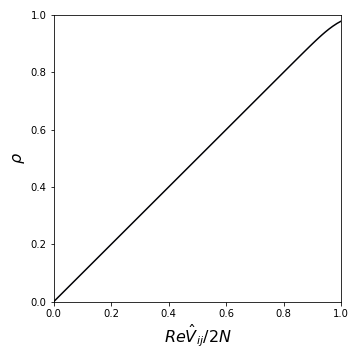
\includegraphics[width=80mm]{corrtestplot4.png}
\caption{The cross-correlation Van Vleck correction function (equation~\ref{crosscorr}) plotted with $\sigma_1=1.0, \sigma_2=1.0$.\label{corrplot}}
\end{figure}

\begin{figure}
\centering{}
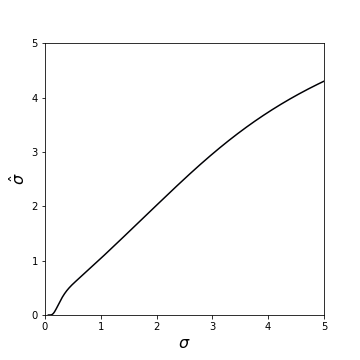
\includegraphics[width=80mm]{sigmatestplot4.png}
\caption{The auto-correlation Van Vleck correction function (equation~\ref{autocorr}).\label{sig}}
\end{figure}

\paragraph{}The correction algorithm has a high computational cost associated with equation \ref{crosscorr}, which has $14^2$ exponential terms in the summation. By combining redundant terms, this number can be reduced by a factor of 2. Evaluation of the integral using \texttt{scipy.integrate.quad} requires ~750 computations of the summation. Using a \texttt{scipy} root-finding function proved useful for finding the input of equation \ref{autocorr} given some output. However, this same function is too costly when correcting the cross-correlations, even though only ~5 evaluations of equation \ref{crosscorr} were required for the root-finding function to converge. An additional cost is memory usage, as running the root-finding function requires generation of a Jacobian matrix the size of which is dictated by the number of cross-correlations being corrected. This places a limit on the number of values which can be corrected simultaneously. 
\paragraph{} 
There are several possible solution for mitigating the cost of correcting the cross-correlations. One is to implement a \texttt{scipy} integration function which allows for vectorized integral evaluation, though this has potential for loss in precision. Additionally, moving from a root-finding algorithm to a lookup table might be more computationally efficient. Both root-finding and a lookup table may ultimately require parallelization to be feasible. Another, perhaps more complicated but also potentially interesting, alternative is to exploit the role of the corrected auto-correlations in equation \ref{crosscorr} and use the shapes of the correction on the autos to determine the shape of the correction on the respective cross-correlation. 
\appendix
\section{Circular Complex Gaussian Random Variables}\label{ccrv}
\paragraph{}A circular complex random variable $Z=\Re(Z)+i\Im(Z)$ is defined as having a distribution that is invariant under a random phase shift:
\begin{align}
E[Z]&=E[e^{i\phi}Z]=0,\\
E[ZZ]&=E[e^{i\phi}Ze^{i\phi}Z],\\
E[ZZ^*]&=E[e^{i\phi}Ze^{-i\phi}Z^*]].
\end{align}
The last of these conditions is trivial. The first and second are only satisfied if $E[Z]=E[ZZ]=0$. Thus
\begin{align}
E[ZZ]&=0\\
&=E[(\Re(Z)+i\Im(Z))(\Re(Z)+i\Im(Z))]\\
&=E[\Re(Z)^2]-E[\Im(Z)^2]+iE[\Re(Z)\Im(Z)]+iE[\Im(Z)\Re(Z)]
\end{align}
and
\begin{align}
E[\Re(Z)^2]&=E[\Im(Z)^2],\\
E[\Re(Z)\Im(Z)]&=-E[\Im(Z)\Re(Z)]=0\label{CC1}.
\end{align}
For a complex random variable, the variance $\sigma_Z^2=E[ZZ^*]=E[\Re(Z)^2]+E[\Im(Z)^2]$. So in the case of a circularly complex random variable
\begin{equation}
\sigma_Z^2=2E[\Re(Z)^2]=2E[\Im(Z)^2].
\end{equation}
Two circular complex random variables sampled from the same distribution have the following relations
\begin{align}
E[\Re(Z_1)\Re(Z_2)]&=E[\Im(Z_1)\Im(Z_2)]\\
E[\Re(Z_1)\Im(Z_2)]&=-E[\Im(Z_1)\Re(Z_2)]\label{CC2}
\end{align}
If this relation does not hold for circular complex random variables sampled from different distributions, then some assumptions are required for the correlator input model.
\paragraph{}For example, consider the case of a correlator input $Z=S+N$, where $S$ and $N$ are both circular complex Gaussian random variables, that is, in addition to the conditions above, the real and imaginary parts of $S$ and $N$ are sampled from zero-mean Gaussian distributions. To treat $Z$ as circularly complex requires $E[\Re(Z)\Im(Z)]=0$. Thus
\begin{equation}
E[\Re(S)\Im(S)]+E[\Re(N)\Im(N)]+E[\Re(S)\Im(N)]+E[\Re(N)\Im(S)]=0.
\end{equation}
The first two terms vanish according to \eqref{CC1}. If \eqref{CC2} applies to circular complex random variables sampled from different distributions, the last two terms vanish. If the relation does not apply, then it is required that $E[\Re(S)\Im(N)]=E[\Re(N)\Im(S)]=0$, that is, that the sky signal and receiver noise are uncorrelated. 
\nocite{*}
\printbibliography
%\bibliographystyle{apsrmp4-2}
\end{document}